\section{Assignment 2. Linear regression.}

\subsection{Selection of features}

First of all, let's take a look at all continuous features' scatterplot to indentify which of them are linear dependent. 
Some features have nearly log-normal distributions, so, for more accurate and reliable linear regression we will logarithm these features.

\begin{figure}[h!]
 \begin{center}
    \center 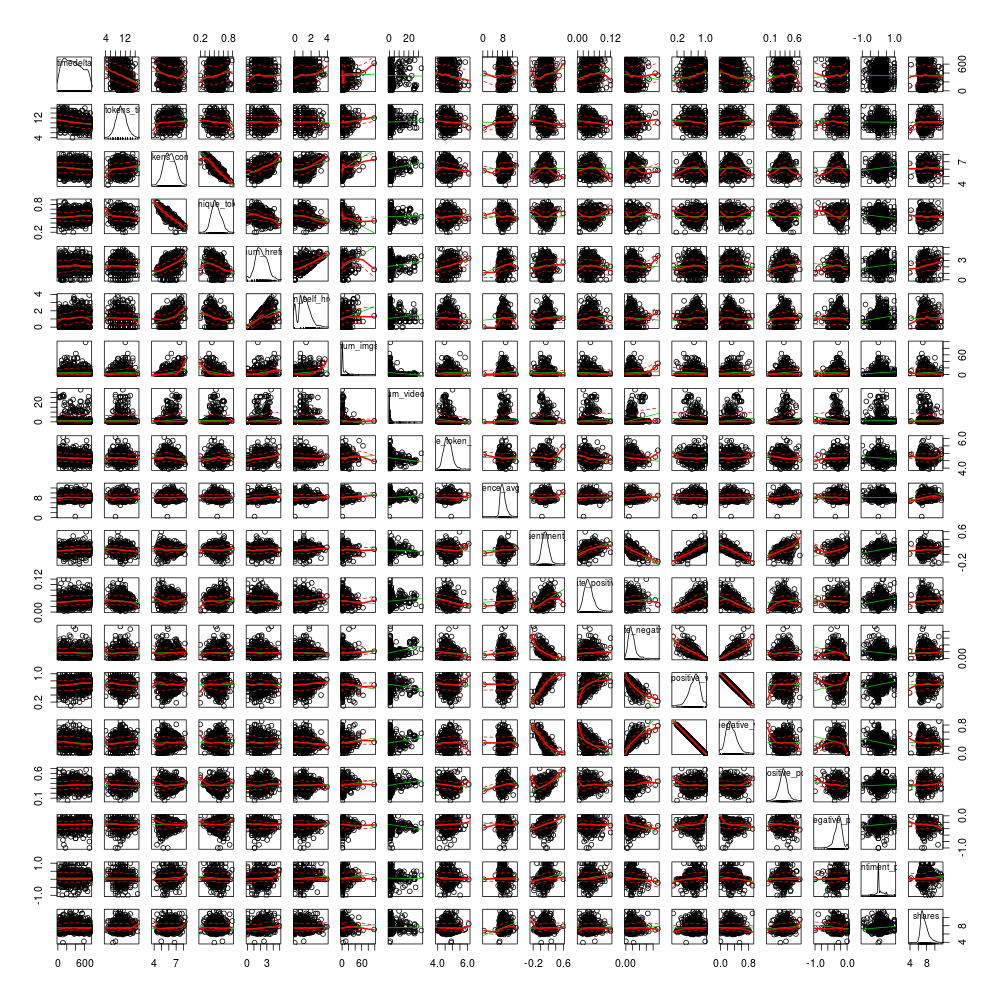
\includegraphics[width = 0.9\textwidth]{scatterplot_matrix_continuous_features_logged.png}
   \caption{Scatterplot matrix of all considered continuous features}
   \label{img:scatterplot_matrix_continuous_features_logged}
 \end{center}
\end{figure} 

As we can see from the scatterplot, the majority of pairs are not linear dependent. Fortunately, \texttt{global\_sentiment\_polarity} and \texttt{rate\_positive\_words} are linear dependent and we can easily understand why: they measure practicaly the same characteristic. The first feature is normalized from 0 to 1 (in out data from 0 to 0.7), the second one takes values from 0 to 1.

We will predict sentiment polarity over positive words rate. As we have rather heterogeneous data, let's make sure we won't be able to do our regression better with the help of groupping by \texttt{Channel} (Figure \ref{img:scatterplot_ratepositive_polarity}, a).

\begin{figure}[h]
\begin{minipage}[h]{0.49\linewidth}
\center{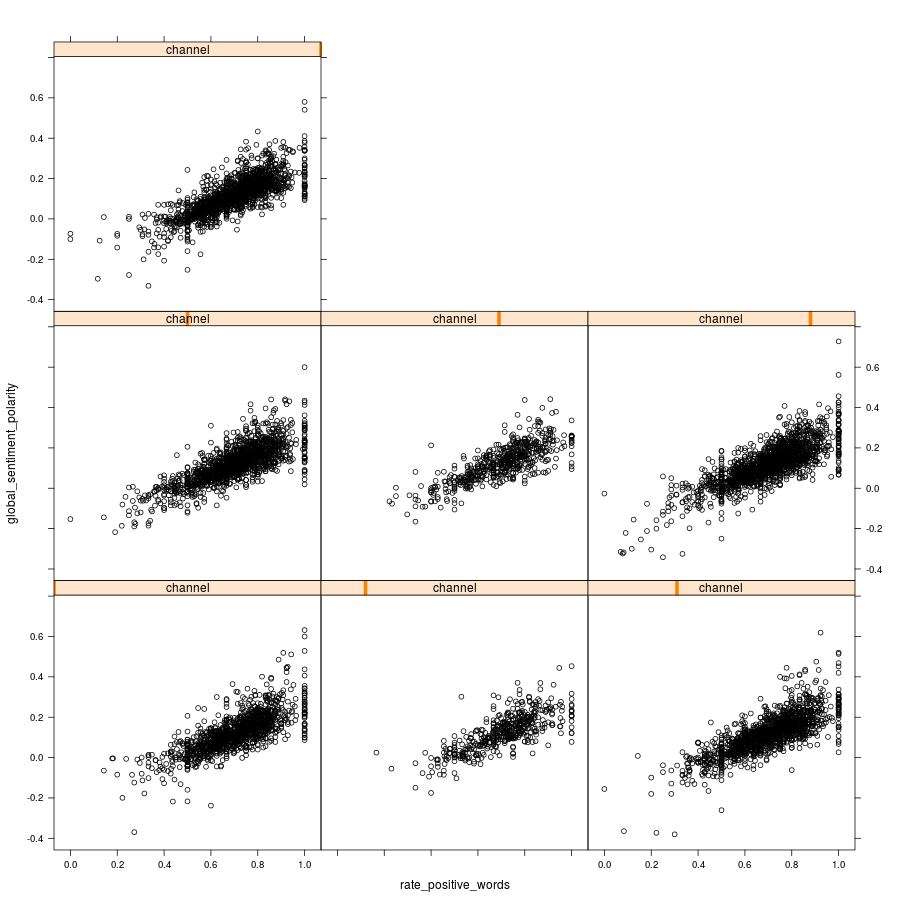
\includegraphics[width=0.95\linewidth]{scatterplot_ratepositive_polarity_groupped.png} \\ a)}
\end{minipage}
\hfill
\begin{minipage}[h]{0.49\linewidth}
\center{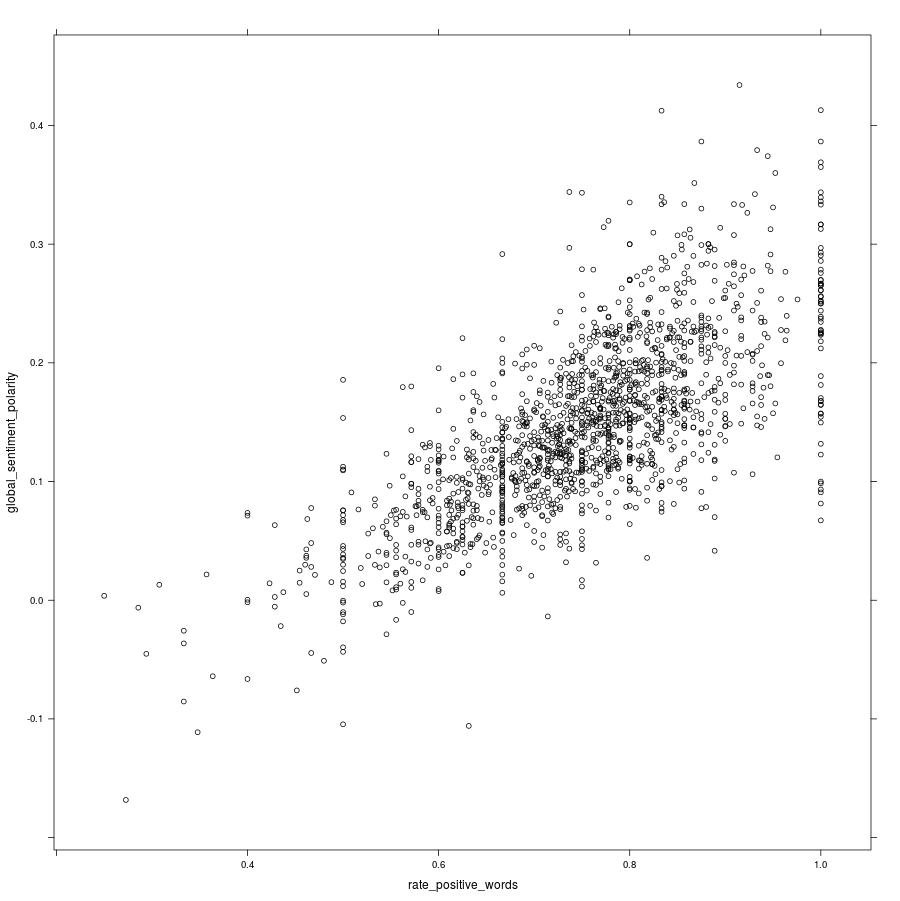
\includegraphics[width=0.95\linewidth]{scatterplot_ratepositive_polarity.png} \\ b)}
\end{minipage}
\caption{Groupped by channel (a) and only technical channel (b) dependece between \texttt{global\_sentiment\_polarity} and \texttt{rate\_positive\_words}.}
\label{img:scatterplot_ratepositive_polarity}
\end{figure}

All chanells looks very similar, and we dicided to consider only technical channel (just to reduce the sample size). After all these actions our scatterplot looks like at (Figure \ref{img:scatterplot_ratepositive_polarity}, b). Further at this section we will call the predicted and the prediction features just \texttt{global\_sentiment\_polarity} and \texttt{rate\_positive\_words}, implying we work with only one channel.
 
\subsection{Model of linear regression}

Using basic functions in R, we have built a linear regression with slope equals 0.4341 and intercept equals  -0.1788. The results of the regression you can see in Figure \ref{img:scatterplot_lr_ratepositive_polarity}.

\begin{figure}[h!]
 \begin{center}
    \center 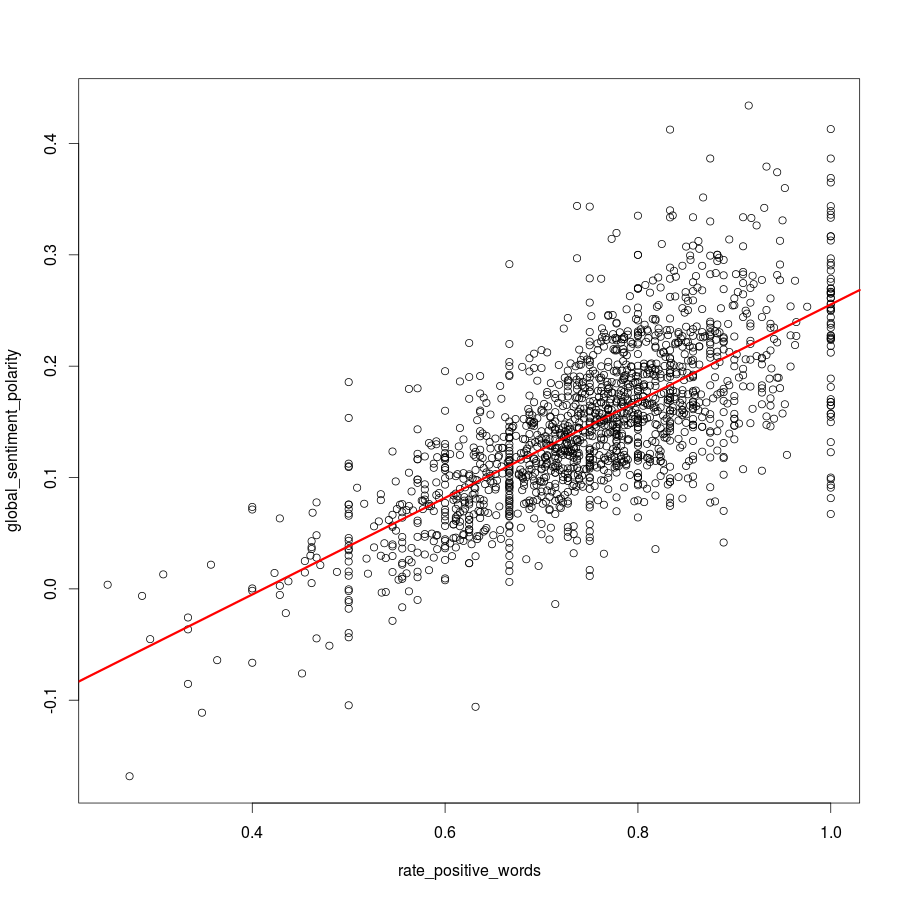
\includegraphics[width = 0.9\textwidth]{scatterplot_lr_ratepositive_polarity.png}
   \caption{}
   \label{img:scatterplot_lr_ratepositive_polarity}
 \end{center}
\end{figure} 

The slope is significantly positive (p-value equals 0) and it's not surpising: the more positive words are in the article, the more text is of positive polarity.

\subsection{Correlation and determinacy coefficients}

The correlation equals 0.7170736 and the coefficient of determination equals 0.5142 (ajusted is 0.5139). As we know from the definition of the coefficient of determination, $R^2$ measures of how well the regression line approximates the real data points and equals the ratio of explained variance. It's believed in practice that $R^2 > 0.5$ is acceptable, but not enough accurate. 

Particularly the value of 0.5139 means that about 51\% of variablility between the two   \texttt{global\_sentiment\_polarity} and \texttt{rate\_positive\_words} is captured by the linear model built with linear regression and the remaining 49\% of variability still remains unaccounted for. 

In another words the value of determination coefficient $R^2$ shows the rate of decrease of the variance of \texttt{global\_sentiment\_polarity} after its linear relation to \texttt{rate\_positive\_words} has been taken into account by the regression.

\subsection{Bootstrap}
We have conducted 5000 boostrap trials to estimate 95\%  confidence intervals of slope, intercept and correlation coefficient. 
The results are summarized by the histograms shown in the figures \ref{fig:bootsrap_intercept}-\ref{fig:bootsrap_correlation}. 

It can be easily seen that histograms are pretty similar to the normal type of distribution.  But let us prove that. 

We have  performed   the  Shapiro-Wilk normality test with intercept, slope and correlation coefficient bootstrap distributions. The results shown in the Table \ref{tbl:p_test_shapir_wilks}  are a little bit striking: with good p-value it is  trustworthy that intercept and slope boostrap samples are obtained from the normal distribution, but we could not say so about correlation coefficient samples data.

So for the correlation coefficient we compute CI using ranked quntiles.
The aforesaid results we  obtained are shown  in Table \ref{tbl:conf_intervals_intercept_slope_corr}.
It is worth to mention that the difference in estimating correlation coefficient CI using the assumption of normallity and without such is not very huge, but we think it is a good idea not only test normality of the data by it's visualization but also with statistical tests.

\begin{table}
	\centering
	\caption{Shapiro-Wilk normallity test p-value} \label{tbl:p_test_shapir_wilks} 
	\begin{tabular}{|c|c|}
		\hline  & 95\%  p-value \\ 
		\hline Intercept & 0.2279 \\ 
		\hline Slope  & 0.244  \\ 
		\hline Correlation &  5.621e-08 \\ 
		\hline 
	\end{tabular} 
\end{table} 




\begin{table}
\centering
	\caption{95\% confidence intervals (CI's) for intercept, slope, correlation coefficient based on bootrap techinque} \label{tbl:conf_intervals_intercept_slope_corr} 
\begin{tabular}{|c|c|}
	\hline  & 95\%  CI \\ 
	\hline Intercept &  (-0.209; -0.148) \\ 
	\hline Slope  & (0.392;  0.476)  \\ 
	\hline Correlation (normal) & (0.668; 0.765)   \\ 
	\hline Correlation (percentile) & (0.666,  0.763)   \\ 
	\hline 
\end{tabular} 
\end{table}
 
\begin{figure}[h!]
\centering
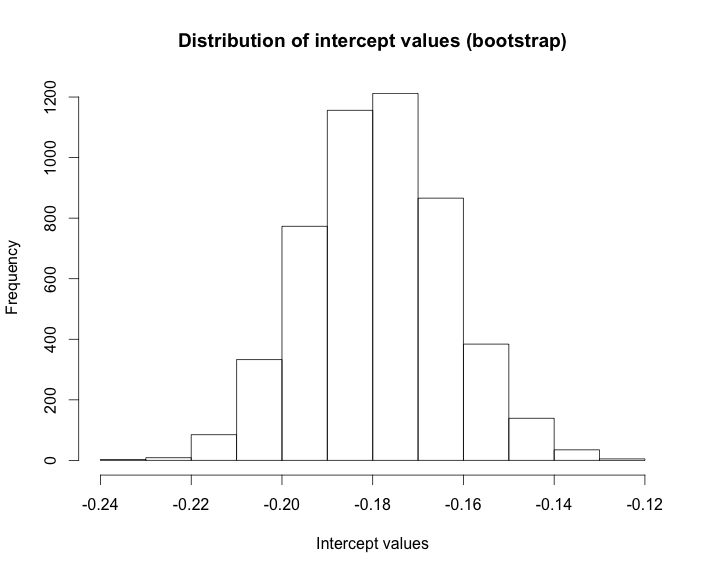
\includegraphics[width=0.7\linewidth]{images/bootsrap_intercept}
\caption{Distribution of intercept value of linear regression models built with each pair of sampled (\texttt{global\_sentiment\_polarity})  and  (\texttt{rate\_positive\_words}) using bootrsap}
\label{fig:bootsrap_intercept}
\end{figure}


\begin{figure}[h!]
\centering
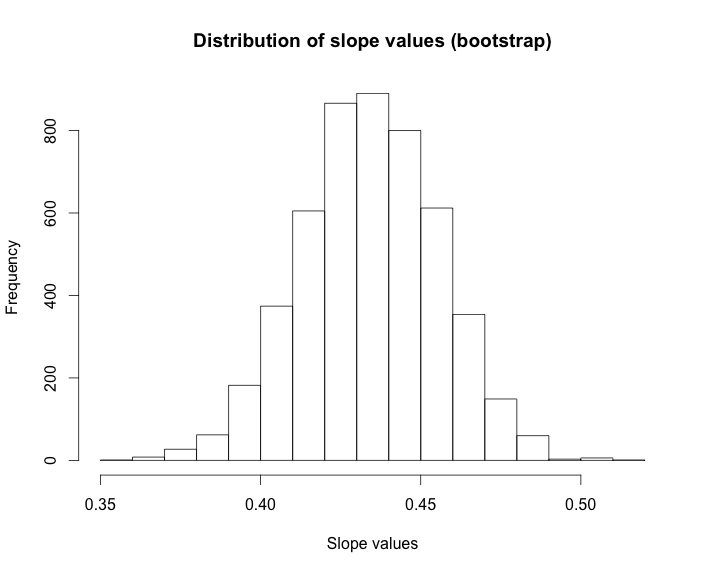
\includegraphics[width=0.7\linewidth]{images/bootsrap_slope}
\caption{Distribution of slope value of linear regression models built with each pair of sampled (\texttt{global\_sentiment\_polarity})  and  (\texttt{rate\_positive\_words}) using bootrsap}
\label{fig:bootsrap_slope}
\end{figure}



\begin{figure}[h!]
\centering
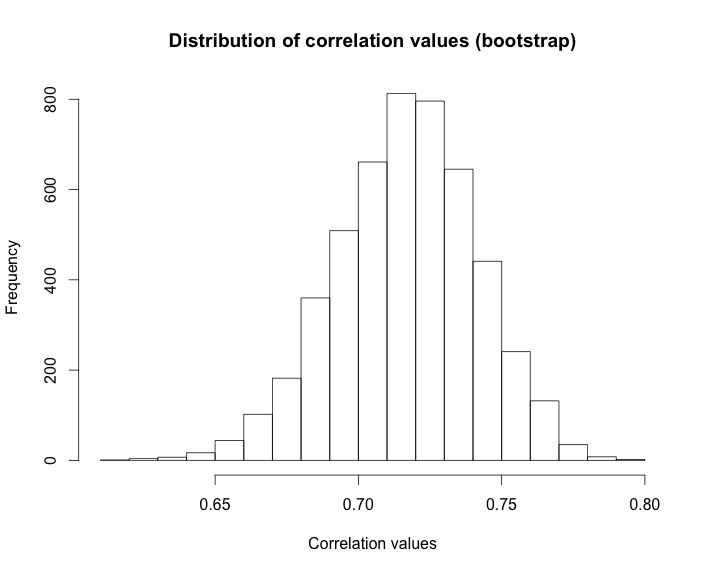
\includegraphics[width=0.7\linewidth]{images/bootsrap_correlation}
\caption{Distribution of correlation values between dependent variable (\texttt{global\_sentiment\_polarity}) and regressor (\texttt{rate\_positive\_words})}
\label{fig:bootsrap_correlation}
\end{figure}



\subsection{Average relative error}

Recall average relative error (ARE) and coefficient of determination (R$^2$) definitions:
\begin{gather*}
\text{ARE} = \frac{1}{N} \sum_{i=1}^{N}{\left\vert \frac{y_i - \hat{y}_i}{y_i} \right\vert}, \\
\text{R}^2 = 1 - \frac{\sum\limits_{i=1}^n (y_i - \hat{y}_i)^2}
                      {\sum\limits_{i=1}^n (y_i - \bar{y})^2}
\end{gather*}


\begin{lstlisting}[language=R]
mean( abs((y.feature - model$fitted.values)/y.feature) * 100) # in %
> 56.37 
summary_regression$r.squared * 100 # in %
> 51.419 
\end{lstlisting}

As we can see, considered values are reasonably close. But we should note that ARE is sensitive to the addition of a constant to all of the $y_i$ while R$^2$ is not. That is, we could obtain any arbitrary value of ARE keeping the coefficient of determination constant by adding some constants to $y_i$. 

It was suprise to us that ARE can be greater than 1 (which is the case if $y_i$ is much less than $y_i - \hat{y}_i$). 

According to all these facts one could conclude that comparing ARE and R$^2$  is meaningless without additional assumptions.


\subsection{Nature-inspired algorithm}
We will use nature-inspired algorithm to compute the parameters of linear regression that minimize the absolute relative error. If the target values of regression are $y_i$ and predicted by linear regression values are $\hat{y}_i$, the  absolute relative error is:
\begin{equation}
\frac{1}{N} \sum_{i=1}^{N}{\left\vert \frac{y_i - \hat{y}_i}{y_i} \right\vert}.
\end{equation}

We have implemented algorithm similar to the one, which is described in \cite{CCODA_Mirkin}, but we will minimize the function \texttt{delta(coefficients, x, y)}, which looks like
\begin{lstlisting}[language=R]
delta <- function(coefficients, x,y){
  a = coefficients[1]; b = coefficients[2]
  yp <- a*x + b
  esq <- mean( abs((y - yp)/y) ) 
} 
\end{lstlisting}

We also need the function that compute permissible limits for coefficients. Let look at two values of target $y_i = a \cdot x_i + b$ and $y_j = a \cdot x_j + b$ ($i \neq j$) and express $a$, $b$ in terms of $x$ and $y$:
\begin{equation*}
a_{ij} = \frac{y_j - y_i}{x_j - x_i}, \ b_{ij} = \frac{y_i x_j - y_j x_i}{x_j - x_i}.
\end{equation*}
And then we calculate $\max$ and $\min$ of coefficients $a$ and $b$ among all pairs $(x_i,y_i)$ and $(x_j,y_j)$. 

%That implemented in the function \texttt{ddr(x, y)}.  The code of this function and function \texttt{nlr(x,y, popSize = 15, iter = 5000)} is given below.

Using the nature-inspired approach (we have implemented it in R-function nlr) we obtained the following values
of slope ($a$) and intercept ($b$) and value of relative error:
\begin{lstlisting}[language=R]
# The regression model: y.feature = a * x.feature + b
# Coefficients of slope and intercept respectively:
model.nlr <- nlr(x.feature, y.feature) 
> 0.3514270 -0.1421007

# Value of relative error:
eps.nlr <- y.feature - model.nlr[1]*x.feature - model.nlr[2]
mean( abs(eps.nlr / y.feature) ) * 100
> 50.54
\end{lstlisting}

Comparing the values of two relative errors, we can see that nature-inspired approach reduce its value by a few percent. 
%
%The main code of nature-inspired approach:
%\begin{lstlisting}[language=R]
%# ddr determine the permissible limits for slope and intercept 
%ddr <- function(x,y){
%  ll <- length(x)
%  eps <- 0.05
%  a <- ldply(1:(ll-1), function(i){
%    v <- sapply((i+1):ll, function(j) 
%      ifelse(abs(x[i] - x[j]) > eps, 
%        (y[i] - y[j])/(x[i] - x[j]), NA))
%    c(min(v, na.rm = TRUE), max(v, na.rm = TRUE))
%  })
%  b <- ldply(1:(ll-1), function(i){
%    v <- sapply((i+1):ll, function(j) 
%      ifelse(abs(x[i] - x[j]) > eps, 
%        (y[j]*x[i] - y[i]*x[j])/(x[i] - x[j]), NA))
%    c(min(v, na.rm = TRUE), max(v, na.rm = TRUE))
%  })
%  
%  list(a.boundaries = c(min(a[,1]), max(a[,2])), 
%       b.boundaries = c(min(b[,1]), max(b[,2])))
%}
%
%# Realization of nature-inspired approach
%# The code is similar to the Matlab code from CCODA textbook 
%nlr <- function(x,y, popSize = 15, iter = 5000){
%  ll <- length(x)
%  bounds <- ddr(x,y) #intervals for coefficients
%  lb <- c(bounds[[1]][1],bounds[[2]][1])
%  rb <- c(bounds[[1]][2],bounds[[2]][2])
%  feas <- matrix(c(rep(rb[1]-lb[1],popSize),rep(rb[2]-lb[2],popSize)),
%   ncol=2) * cbind(rnorm(popSize),rnorm(popSize)) +
%       matrix(c(rep(lb[1],popSize), rep(lb[2],popSize)), ncol = 2)
%  flag = 1; count = 0; funp = 0
%  vv <- apply(feas, 1, function(d) delta(d, x, y))  
%  funi <- min(vv); ini <- which.min(vv); soli <- feas[ini,]
%  si = 1
%  while (flag == 1){
%    count <- count + 1
%    feas <- feas + cbind(rnorm(popSize),rnorm(popSize))
%    feas <- t(apply(feas, 1, function(x) ifelse(x > lb, 
%              ifelse(x < rb, x, rb), lb)))
%    vec <- apply(feas, 1, function(d) delta(d, x, y)) 
%    fun <- min(vec); un <- which.min(vec); sol <- feas[un,]
%    wf <- max(vec); wi <- which.max(vec); wun <-feas[wi,]
%    if (wf > funi){
%      feas[wi,] <- soli 
%      vec[wi] <- funi
%    } 
%    if (fun < funi) {
%      soli <- sol; funi <- fun
%    }
%    if (count >= iter) { flag = 0 }
%    residvar <- funi/var(y)
%  }
%  a <- soli[1]; b <- soli[2]
%  c(a,b)
%}
%\end{lstlisting}

In R-language there is a package \texttt{genalg} with function \texttt{rbga} that implement this approach. The results obtained with function \texttt{rbga} are very close to the results described above:
\begin{lstlisting}[language=R]
# The regression model: y.feature = a * x.feature + b
# Calculate the permissible limits for a and b 
bound <- ddr(x.feature, y.feature)
bounds.min <- c(bound[[1]][1],bound[[2]][1]) # (a.min, b.min) 
bounds.max <- c(bound[[1]][2],bound[[2]][2]) # (a.max, b.max)

rbga.res <- rbga(bounds.min, bounds.max, popSize = 30, iters = 5000,
   evalFunc = function(coefs) delta(coefs, x.feature, y.feature))

# Results (we need to take a look at "Best Solution")
summary(rbga.res)
> GA Settings
  Type  = floats chromosome
  Population size       = 30
  Number of Generations = 5000
  Elitism               = 6
  Mutation Chance       = 0.333333333333333
  
  Search Domain
  Var 1 = [-6.674999999946,6.47188552188199]
  Var 2 = [-5.27885519411197,5.97499999995278]
  
  GA Results
  Best Solution : 0.347731933975272 -0.146302152742407 

# Value of relative error:
delta(c(0.3477, -0.1463), x.feature, y.feature)) * 100
> 49.93
\end{lstlisting}